%% --------------------------------------------------------
%\documentclass[preprint2]{aastex}
\documentclass[12pt,preprint]{aastex} 

%\documentclass{emulateapj}
\usepackage{lineno} 
\usepackage{natbib}
\usepackage{epsf}
\usepackage{url}
\usepackage{color}
\usepackage{mathrsfs}
\citestyle{aa}
%% --------------------------------------------------------
\newcommand{\tc}[2]{\textcolor{#1}{#2}}
\newcommand{\Msun}{\ifmmode\mbox{M}_{\odot}\else$\mbox{M}_{\odot}$\fi}
\newcommand{\Rsun}{\ifmmode\mbox{R}_{\odot}\else$\mbox{R}_{\odot}$\fi}
\newcommand{\Mearth}{\ifmmode\mbox{M}_{\oplus}\else$\mbox{M}_{\oplus}$\fi}
\newcommand{\Rearth}{\ifmmode\mbox{R}_{\oplus}\else$\mbox{R}_{\oplus}$\fi}
\newcommand{\msR}{\mathscr{R}}
\def\bfref{\color{red}}
%\newcommand{\Mark}{\bf \textcolor{r}}
%\newcommand{\chandra}{\textit{Chandra}\,}
%\newcommand{\spitzer}{\textit{Spitzer}\,}
%%\newcommand{\xmm}{\textit{XMM-Newton}\,}
%\newcommand{\xmm}{\textit{XMM}\,}
%\newcommand{\xte}{\textit{RXTE}\,}
%\newcommand{\rosat}{\textit{ROSAT}\,}
%\newcommand{\ooft}{4U~0142$+$61\,}
%\newcommand{\seven}{RXS~J170849.0$-$400910\,}
%\newcommand{\eight}{1E~1841$-$045\,}
%\newcommand{\etff}{AX~1845$-$0258}
%\newcommand{\etfs}{PSR~J1846$-$0258}
%\newcommand{\ttfn}{1E~2259$+$586}
%\newcommand{\tfe}{1E~1048.1$-$5937\,}
%\newcommand{\etten}{XTE~J1810$-$197\,}
%\newcommand{\ninet}{SGR~1900$+$14}
%\newcommand{\etos}{SGR~1806$-$20\,}
%\newcommand{\ntst}{PSR~B1916$+$14\,}
%\newcommand{\stet}{PSR~J1718$-$3718\,}

\shorttitle{21 years timing of PSR J1713+0747.}
\shortauthors{Zhu et al.}

%% --------------------------------------------------------
%% \slugcomment{Submitted to ApJ}
%% --------------------------------------------------------
\begin{document}
%% --------------------------------------------------------
\title{21-Year Timing of Millisecond pulsar J1713+0747 with Arecibo and GBT}

%% --------------------------------------------------------
\author{
W. W. Zhu\altaffilmark{1},
I. H. Stairs\altaffilmark{1},
P. B. Demorest\altaffilmark{2},
D. J. Nice\altaffilmark{3},
S. M. Ransom\altaffilmark{2},
Z. Arzoumanian\altaffilmark{4,5},
K. Crowter\altaffilmark{1},
T. Dolch\altaffilmark{6},
R. D. Ferdman\altaffilmark{7}, 
E. Fonseca\altaffilmark{1}, 
M. E. Gonzalez\altaffilmark{8}, 
G. Jones\altaffilmark{2,9}, 
M. T. Lam\altaffilmark{6}, 
L. Levin\altaffilmark{10}, 
M. A. McLaughlin\altaffilmark{10}, 
T. Pennucci\altaffilmark{2}, 
K. Stovall\altaffilmark{11}, 
J. Swiggum\altaffilmark{10}
}
%% --------------------------------------------------------
%% \email{}
%% --------------------------------------------------------
\altaffiltext{1}{\footnotesize Department of Physics and Astronomy,
6224 Agricultural Road, University of British Columbia, Vancouver, BC, V6T 1Z1, Canada;
zhuww@phas.ubc.ca, istairs@phas.ubc.ca}
\altaffiltext{2}{\footnotesize NRAO, Charlottesville, VA 22903, USA}
\altaffiltext{3}{\footnotesize Department of Physics, Lafayette College,
Easton, PA 18042, USA}
\altaffiltext{4}{\footnotesize Center for Research and Exploration in Space Science and
Technology and X-Ray Astrophysics Laboratory, NASA Goddard Space Flight
Center, Code 662, Greenbelt, MD 20771, USA}
\altaffiltext{5}{\footnotesize Universities Space Research Association, Columbia, MD 21044,
USA}
\altaffiltext{6}{\footnotesize Department of Astronomy, Cornell University, Ithaca, NY
14853, USA}
\altaffiltext{7}{\footnotesize Department of Physics, McGill University, Montreal, QC H3A
2T8, Canada}
\altaffiltext{8}{Department of Nuclear Medicine, Vancouver Coastal Health
Authority, Vancouver, BC V5Z 1M9, Canada}
\altaffiltext{9}{\footnotesize Department of Physics, Columbia University, 550
W. 120th St. New York, NY 10027, USA}
\altaffiltext{10}{\footnotesize Department of Physics, West Virginia University, P.O. Box
6315, Morgantown, WV 26505, USA}
\altaffiltext{11}{\footnotesize Department of Physics and Astronomy, University of New
Mexico, Albuquerque, NM, 87131}

%% --------------------------------------------------------
%\begin{abstract}
%\end{abstract}

%% --------------------------------------------------------
\keywords{pulsars: individual (\object{PSR J1713+0747}) --- Radio: stars --- stars: neutron
--- Binaries:general --- gravitation -- relativity}

%% --------------------------------------------------------
%% A small citation guide:
%% \citep{jon90} (Jones et al. 1990) [no comma] 
%% \cite(t){jon90} Jones et al. (1990) [no comma]
%%
%% \citep*{jon90} (Jones, Baker, and Williams 1990) [one arg, no comma]
%% \citet*{jon90} Jones, Baker, and Williams (1990) [one arg]
%%
%% \citealp(jon90) Jones et al. 1990  [no comma]
%% \citealt{jon90} Jones et al. 1990  [no comma, been using this]
%%
%% \citealp*{jon90} Jones, Baker, and Williams 1990 [all and no comma,this]
%% \citealt*{jon90} Jones, Baker, and Williams 1990 [all and no comma]
%% --------------------------------------------------------



\begin{abstract}
Pulsars are precise cosmic clocks and excellent testing grounds for
fundamental physics, especially for testing
gravitational theories. We report 21-year timing of one of the most precise
pulsars: PSR~J1713+0747. The pulse times of arrival of this pulsar are well
modeled by a comprehensive binary model, which included the 3-D orientation 
of the orbit in the sky, with residuals of estimated variance of $\sim 210$~ns. 
We also measured the binary orbit's apparent decay due to motion 
between the pulsar and the observer. Our results set
a limit on the change rate of the gravitational constant $\dot{G}$. 
%as predicted in some alternative theories of strong-field gravity. 
$\dot{G}$ is found to be consistent with zero and at 
least a factor of $43$ (99.7\% confidence level) slower than the average expansion 
rate of the Universe. Such a limit has important implications for
alternative theories of gravitation.
\end{abstract}


\section{Introduction}
\label{sec:intro}
\linenumbers
We present 21-year timing of the millisecond pulsar PSR~J1713+0747. This pulsar was discovered in 1993 \citep{fwc93} using the largest telescope in the world, the Arecibo telescope. It is one of the brightest pulsars timed by the
North American nano-Hertz Observatory for Gravitation Waves (NANOGrav;
\citealt{ndf+12, dfg+13}), has the smallest timing residual of all NANOGrav
pulsars \citep{dfg+13}, and is one of the best-timed pulsars in the world.
Observations of this pulsar were reported previously in
\citealt{cfw94},\citealt{ vb03}, \citealt{sns+05}, \citealt{hbo06} and \citealt{ver09}.

%The high timing precision and the long base line allowed us to precisely 
%measure the pulsar binary's orbit, masses, distance, proper motion, 
%and orientation on the sky (see Section \ref{sec:model} for
%details). 

Millisecond pulsars (MSPs) are very stable rotators thanks to their enormous angular momentum. PSR~J1713+0747 is one of the most stable MSPs, and it resides in a wide binary orbit with a white dwarf companion (Section \ref{sec:model}). 
The latest wide-bandwidth and high-resolution instruments allow us to model and account for the variation in the interstellar medium (ISM)
(Section \ref{sec:dmx}) and small distortions of the pulsar's magnetosphere (Section \ref{sec:FD}). 
The pulse arrival times of the pulsar are well fit by a binary model with
a nearly circular orbit that is edge on to our line of sight. The masses of
the system components can be inferred through the measurement of Shapiro delay. 
The system's distance is well-measured through timing parallax. We also detect
a changing projected orbital semi-major axis due to the orbit's proper motion
on the sky. Through the change rate of projected semi-major axis, we can infer 
the orientation of the orbit in the sky.
This is one of the only few systems in which the 3D-orientation of the
binary orbit can be completely solved. Using 21 years of data, we
refine the previously-published measurements of these orbital parameters.
%These measurements also enable better tests of the theories of gravitation (see Section \ref{sec:res} for details).

The stability and long orbital period of the PSR~J1713+0747 binary make it the
perfect laboratory for observing the smallest cosmic variance, 
one such as the time variation of Newton's gravitational ``constant'' $G$. 
This interesting conjecture of $G$ varying in a cosmological timescale was first 
raised by \citet{dir37} based on his large-number hypothesis, and 
revisited later by gravitational theories involving extra dimensions
\citep{mar84,ww86a}.
In this paper, we seek to constrain the time variation of $G$ using pulsar
binary in the framework of one of the last remaining alternative theories of gravitation, the scalar-tensor theory \citep{jor59,fie56,bd61}. 
This theory modifies Einstein's equation of gravitation by coupling mass with
a large-scale scalar-tensor field, and predicts that, as the universe expands,
the scalar field will also expand, causing the gravitational constant to vary  
in the cosmological timescale. 
PSR~J1713+0747 is likely the best pulsar binary for testing the constancy of
$G$ thanks to its high timing precision and long orbital period. Using timing
results reported in this paper, we found a stringent upper limit on the
$\dot{G}$ (see Section \ref{sec:Gdot} for detail). 
%like Luna Earth binary or pulsar
%binaries in the matter of decades. The Luna Laser Ranging (LLR) experiment measured the
%Luna-Earth distance to $10^{-11}$ precision for a 39 years time span, and thus put a very good upper limit on the change rate of gravitational constant
%\citep{hmb10}. Recently, thanks to the high-precision pulsar time array
%projects, measurements of pulsar binary orbits have also been improved
%greatly, reaching similar precision as the LLR experiment and start to provide
%meaningful independent constrains on $\dot{G}/G$. PSR J1713+0747 is uniquely
%useful in this particular test, because of its long orbital period. Unlike in
%other pulsar binaries, where the orbital decay could be affected by
%gravitational wave radiation (as predicted by Einstein's GR or by 
%alternative theories), this system has very small gravitational radiations. 
%Therefore, it is likely the best system for testing the constancy of
%gravitational constant. We found that by combining the timing result of
%J1713+0747 with that of other pulsars', we get a significantly 
%improved upper limit on $\dot{G}/G$ compare with previous timing-based 
%limits (see Section \ref{sec:Gdot} for detail).

The PSR~J1713+0747 binary is also an excellent laboratory for testing physical 
principles such as the strong equivalence principle (SEP) and the Lorentz invariance, because small violation of these principles could polarize the
binary orbit and result in potentially observable effects. We can set
upper limits on the violations of these principles by observing
low-eccentricity pulsar binary systems. Section \ref{sec:sep} presents the
constraint on the violation of SEP and Lorentz invariance from our 21 years of observation of PSR~J1713+0747.

\section{Observations}
Timing observations of PSR~J1713+0747 started in 1993 at the Arecibo
Observatory. Long-term timing programs started observing the pulsar in
late 1998, with the direct detection of GW as a partial
motivation. \citet{sns+05} reported the results of the first 12 years
of timing observations. Since 2005 the pulsar is observed monthly
at 1400~MHz and 2300~MHz by the Arecibo
observatory and at 800~MHz and 1400~MHz by the Robert C. Byrd Green Bank
Telescope (GBT; proposal code:GBT12B-320).

The timing observations were conducted 
using multiple generations of pulsar data systems. The early 
observations in \citet{sns+05} used
 the Princeton Mark~III \citep{skn+92} and Mark~IV
\citep{sst+00} instruments, and the Arecibo-Berkeley Pulsar Processor
(ABPP) systems \citep{bdz+97}. 
From 2004 to 2011/12, pulsar data were collected with the Astronomical Signal
Processor (ASP; \citealt{dem07}) and its Green Bank counterpart GASP \citep{dem07},
mostly as part of the formalized North American Nanohertz Observatory
for Gravitational Waves (NANOGrav) project. We
started using 
the Green Bank Ultimate Pulsar Processing Instrument (GUPPI; \citealt{GUPPI}) for GBT 
observations in 2010 and its clone the Puerto-Rican Ultimate Pulsar Processing Instrument
(PUPPI) for Arecibo observations in 2012. 
The date range, number of observation epochs, specifications of the
systems are listed in Table \ref{tab:obs}.

We combine the pulse time of arrivals (TOAs) used in \citealt{sns+05} and those
of the later observations, for a data span of 21 years with a
noticeable gap between 1994 and 1998, during the Arecibo upgrade.
Data timestamps are derived from observatory masers and retrocorrected
to the Universal Coordinated Time (UTC) via GPS and then further
corrected to the TT(BIPM) timescale using the 2012 version BIPM clock corrections with extrapolations to 2013.
The TOAs are measured from the observational data through a series of
steps. First the data are folded, as they were being taken, into pulse
profiles using an ephemeris known to be good enough for predicting the
pulse periodicity for the duration of the observation. The folded
profiles from different frequency channels and sub-integrations are
often summed together to improve the S/N of the profiles.  Orthogonal
polarizations are summed to produce a total-intensity profile.
The summed profiles are then compared with a well-measured standard
pulse profile from the appropriate frequency band. We employ
frequency-domain cross-correlation techniques \citep{tay92} to determine the phase of the pulse peak relative to the midpoint of the observation. The final TOA of a summed profile is then calculated by adding the mid-observation time and the product of pulse period and the measured peak phase.
The flux density of the pulsar in these observations can also be
measured by comparing the signal strength in the data with that of a
calibration observation taken right before or after the pulsar
observation in which a signal with known strength was injected. For
the post-upgrade Arecibo data and all the GBT data, the
flux density of the calibration signal is calibrated every month by
comparing it with an astronomical object of known and constant flux
density, in this case, the AGNs J1413+1509 and B1442+09.




\section{Timing model}
\label{sec:model}
A comprehensive timing model was described by \citet{sns+05},
including the effects of pulsar rotation, astrometry, orbital motion,
Shapiro delay and dispersion due to the ISM.
We employed the pulsar timing tool \textit{TEMPO}
\footnote{\url{http://tempo.sourceforge.net}} and the same
\citet{dd86} (DD) model \citet{sns+05} used to fit for the pulsar's
spin behavior and orbital motions, but used a Markov-Chain-Monte-Carlo
(MCMC) simulation to determine the parameter uncertainties.
The T2 model in \textit{TEMPO2} \citep{hem06} also can be used for modeling this pulsar. We tested the T2 model and found that its best-fit binary parameters are physically consistent with those we found using DD model.
The DMX model was used to fit DM variations caused by changes in the ISM (see Section \ref{sec:dmx} for details). The FD model was used to model profile
evolution in frequency (see Section \ref{sec:FD} for details). 
We used the DE421 solar ephemeris instead of the DE405 used by
\citet{sns+05} for its improved precision on the masses of the Solar system
planets, despite that using DE405 gave us marginally better $\chi^2$
($\Delta\chi^2\sim20$ for 16750 degrees of freedom).
In the pulsar model, we added an extra fitting parameter, the change rate of binary period $\dot{P}_{\rm b}$ to model a previously undetectable change in $P_{\rm b}$. This is described in Section \ref{sec:obdecay}.    
We can confirm that most of the pulsar-binary parameters reported
\citet{sns+05} also successfully describe the 21-year data
set. The new timing model parameters (Table \ref{tab:par}) differ from
those in \citet{sns+05} slightly but consistently within their reported uncertainties.


%\begin{itemize}
%\item T2 model versus DD? confirms that both model gives pretty much consistent results?
%\end{itemize}

\subsection{Mass measurements}
\label{sec:mass}
PSR~J1713+0747's timing model has been significantly improved by the 21-year timing effort.
Most notably, the pulsar and the companion masses have been more precisely measured
(Figure \ref{fig:mass}; Table \ref{tab:par}). The
companion's mass $M_{\rm c} = 0.283\pm0.004$ and the pulsar $M_{\rm PSR}=1.29\pm0.1$ are in good agreement with the previously measured values \cite{sns+05}.
The pulsar's mass is comparable with the distribution of pulsar masses
in other neutron star-white dwarf systems, and in good
agreement with the distribution of pulsar masses found in recycled binaries
\citep{opns12,kkdt13}. The precise measurement of neutron star mass like this
may eventually help us understand the properties of matter in extreme 
density \citep{lat12}.

In the standard picture of binary evolution, a MSP with a low-mass white dwarf companion must have been spun up through accretion when the white dwarf was a giant star filling its Roche lobe. 
This should lead to a strong correlation between the binary period and the mass of the white dwarf companion \citep{rpj+95, ts99a, prp02b}. 
Indeed, this picture has been supported by the measurements of several pulsar
binary systems \citep[e.g.,][]{vbb+01, ktr94, th14}.  
The orbital period and companion mass of PSR~J1713+0747 fits
this correlation very well, thus supporting the standard MSP evolution theory. %Notably, not all MSP companions follow the same orbital period -- companion
%mass relation, for instance, J1903+0327 has an orbit of 95~days but a
%companion of $\sim 1M_{\odot}$ \citep{fbw+11}. Such peculiar systems requires
%more than the simple scenario considered above to explain.

%Some early statistical analysis shows that pulsars 
%might have a very narrow mass distribution 1.35$\pm0.04M_{\odot}$ \citep{tc99}. 
%However, several massive ($\sim2M_{\odot}$) pulsars have been found in recent
%years (J1614$-$2230 1.97$\pm0.04M_{\odot}$\citealt{dpr+10}; J1913+0327
%1.67$\pm0.02M_{\odot}$ \citealt{fbw+11}, J0348+0432 2.01$\pm0.04M_{\odot}$
%\citealt{afw+13}) that clearly out-lie this distribution.

%J1713+0747 appears to be nominal when compared with the early year samples
%despite of its recycling history.


\subsection{DM variation}
\label{sec:dmx}
The DM of a pulsar reflects the amount of free electrons between
the pulsar and the telescopes and it varies because
our sight-line through the turbulent ISM and solar wind is changing as the
pulsar, the Sun, the Earth, and the ISM all move with respect to each other.
The DM variation can affect the timing of high-precision pulsar significantly.

We fit the time-varying DM using the {\it DMX} model in {\it tempo}.
The model groups TOAs taken within ten days and fits for one
best DM value for each group.  The same procedure was carried out in
\citealt{dfg+13}.  This DM fitting was conducted with TOAs from all
instruments except Mark~III, which produced only single-frequency TOAs.

The ten-day grouping is justified based on the cadence of our multi-band
observations.
The Arecibo 1400-MHz and 2300-MHz observations of PSR~J1713+0747 almost
always happen consecutively on
the same day, while the GBT 800-MHz and 1400-MHz observations often take place on different
days spaced by only few days apart.
Therefore, most DM values in our {\it DMX} model were determined by TOAs from
similar epochs and from at least two frequency bands. 

Figure \ref{fig:dmx} shows the DM variation of PSR~J1713+0747 as measured
using {\it DMX} model.
Note that the systematic drop of DM around MJD 53200 is not real; it is due to
the use of different standard pulse profile templates when extracting 
TOAs from the early-year Mark~IV, ABPP data. The DM values inferred from different
profile templates are expected to have a constant offset.
Conversely, the sudden dip and recovery of DM around MJD 54800 is real and probably
due to changes either in the ISM or in the solar winds. This DM dip is also
observed independently by the Parkes observatory \citep{kcs+13}.
There is clear red-noise-like variance in the pulsar's DM with a RMS of
$\sim10^{-4}$. 
%This DM variation may lead to ``red'' timing residuals as discussed in \citealt{kcs+13}.

Note that the first part of this DM curve (MJD$<53200$) in
Figure \ref{fig:dmx}) has much larger uncertainties than the second half.
This is because the relative inferior frequency resolution of the early-year
data. The Mark~IV data in particular have much smaller frequency bandwidth 
compared to the later data (Table \ref{tab:obs}).
Data from the L- and S-band of Mark~IV and ABPP are collapsed in frequency to
form one TOA per band per observation epoch, thus losing frequency resolution
in the respective band. This makes it hard to resolve the profile evolution in
frequency that we see in the later data. When crunching the data in frequency, we
also assume the center frequency of the band is the middle frequency, while the effective center frequency may be different due to pulse
profile evolution and/or scintillation. This procedure is likely to produce TOAs that are slightly offset. We think this may be why the FD and
DMX models cannot completely model the red-noise signal in these TOAs, leaving
an apparent hump in the first part of the DM curve (Figure \ref{fig:dmx}) and 
a similar shape in the 2300-MHz timing residuals from Mark~IV and ABPP (Figure
\ref{fig:res}).

There is a hint of small annual DM variations, part of these variations may be 
related to the varying electron density in the Solar wind as our sight line moves.
The Earth's motion could also causes a projected helical motion through the ISM
that leads to an annual DM variation.
%The peak values of DM are achieved when the
%Earth is on the opposite side of the Sun from the pulsar (***need to
%check this!***), indicating that this effect is likely due to the
%ionized component of the Solar wind.

It has been shown that the DM variation of some pulsars are consistent with
those expected from an ISM characterized by a Kolomgorov turbulence spectrum
\citep{ric90, ktr94, yhc+07, kcs+13, fst14}. In those cases one can calculate the 
structure function of the varying DM: 
\begin{equation}
D_{\phi}(\tau)=\left(\frac{2\pi C}{f^2}\right)\langle [DM(t+\tau)-DM(t)]^2\rangle, 
\end{equation}
where $\tau$ 
is a given time delay, $C=4.148\times10^3$~MHz$^2$pc$^{-1}$cm$^3$s, and $f$ is 
the observing frequency in MHz, and expect 
this function to follow a Kolomgorov power law $D_{\phi}(\tau)=(\tau/\tau_0)^{\beta -2}$, 
where $\beta=11/3$ and $\tau_0$ is a characteristic time scale related to 
the inner scale of the turbulence. The pulsars with DM variation that fits this
theory generally have large but relatively smooth DM variations in timescale of 
years. However, the DM variation of PSR J1713+0747 (Figure \ref{fig:dmx}) does not 
follow the same characterization. It has a large variation around 2009 for few hundreds days,
but not much long-term variation. Therefore, its structure function rejects
a Kolomgorov type spectrum, instead, favors a smaller spectrum index.



\subsection{Timing noise}
\label{sec:noise}
The pulsar timing residuals (Figure \ref{fig:res}) are the residuals left
after we fit the TOAs with our timing model. 
These residuals are likely caused by timing noise, DM variations, radiometer 
noise, and other sources of noise. This section discusses PSR~J1713+0747's
timing noise, i.e. TOA variations due to spin irregularities.

The term ``timing noise'' in pulsar timing generally refers to a pulsar's spin
irregularity, i.e. its long-term deviation from a simple linear slow down. 
Potential causes of irregular spin behavior include unresolved
micro-glitches, internal superfluid turbulence, magnetosphere variations, or external torques caused by matter surrounding the pulsar
\citep{hlk10, ymh+13, ml14}.
Unlike the Gaussian-like noise due to the measurements of the TOAs, the
timing noise accumulates over time, with a ``red'' 
spectrum. Timing noise is often significant in younger pulsars, and often
gives rise to significant high-order frequency polynomials such as
$\ddot{\nu}$, where $\nu$ is the pulsar's spin frequency.

The timing noise of radio pulsars has been studied by \citet{antt94},
\citet{dmhd95}, \citet{mtem97} and later by \citet{hlk10} with large samples. 
%Because every pulsar has its own unique timing behavior, it is
%hard to quantify the level of timing noise.
\citet{antt94} characterized the significance of timing noise using the second
spin derivative $\ddot{\nu}$, because on the scale of a few years many
pulsars show cubic terms in their residuals. They define the noise factor 
\begin{equation}
\label{eq:delta8}
\Delta_8 = \log_{10}\left(\frac{1}{5\nu}|\ddot{\nu}|t^3\right).
\end{equation}
Here $t=10^8$~s$\sim 3$~yr is a fiducial time scale close to their average
observation time span.
Similarly, \citet{mtem97} adopted a generalized Allen Variance (traditionally used in
measuring clock stability) to characterize the timing instability of pulsars:
\begin{equation}
\label{eq:sigmaz}
\sigma_z(\tau) = \frac{\tau^2}{2\sqrt{5}}\langle c^2 \rangle^{1/2},
\end{equation}
where $\langle c^2\rangle$ denote the sum of squares of the cubic
terms fitted to segments of length $\tau$). 
$\Delta_8$ is basically the logarithm of a dimensionless form of $\sigma_z(10^8~s)$.

PSR~J1713+0747's
best-fit $\ddot{\nu}$ (table \ref{tab:par}) is not statistically significant. 
Therefore, there is no evidence of significant timing noise with the
timescale of the 21 years. The only red-noise like
signal is the small hump in the early-year 2300-MHz Mark~IV and ABPP timing
residuals in Figure \ref{fig:res}, and we think it is likely caused by DM variations not resolved in
these data. Figure \ref{fig:TN} 
shows PSR~J1713+0747's $\sigma_z$ values for various timescales, compared 
with the values from simulated residuals containing white noises and
red noises that grow significantly in few years of time
scales. The observed $\sigma_z$ values seem to be more consistent 
with the white-noise simulations, not with the specific red noise
simulation. This suggests that the spin of PSR~J1713+0747 is likely very
regular, as one would expect from an old recycled pulsar in a wide binary
orbit. %with smaller than 1 year of typical timescale. 
This result is also consistent with the timing noise analysis of this pulsar in 
\citet{pjl+13}. They
studied the timing noise using an auto-correlation technique
based on 5 year NANOGrav data, and conclude that the timing residuals are
consistent with mostly white noise.
%The lack of short- and long-timescale red noise suggests the
%deviation from simple spin down could be very small in this pulsar and its timing
%residuals are dominated by Gaussian-like noises such as the radiometer noise.

Note that, \citet{kcs+13} argue that fitting for DM variation in short cadence could
absorb a portion of the noises in the TOAs into the DMX model. 
Indeed, our noise-injection simulation (Section \ref{sec:res})
also show that some noises in the residuals are absorbed by model fitting
including the DM corrections. Although a thorough noise analysis is out of the scope of
this paper.
%Whether the ``absorbed'' signals are ``red'' is not clear.
%Such effect should affect our pre-2005 timing
%residuals more than the post-2005 ones. Because the post-2005 DM variations 
%are well determined by at least two wide band observations, and should
%``absorb'' less frequency independent ``red'' signals.
%Conversely, we observed no obvious increase in noise level in the post-2005
%residuals, which does not support the existence of significant
%frequency independent ``red'' noise.


\subsection{Pulse profile evolution in frequency}
\label{sec:FD}
After removing the dispersion that causes TOA delays of $\propto \nu^{-2}$,
 we still see small remaining frequency-dependent residuals from wide-band
observations using
different instruments and different telescopes (Figure \ref{fig:FD}).  
The cause of such profile evolution is likely a change in the pulsar's
radiation pattern with frequency.  Pulsar radiation of different frequencies may originate from
different parts of the star's magnetosphere, and 
the radiation region of the pulsars's magnetosphere may be slightly distorted,
leading to a frequency-dependent radiation pattern. \citet{pdr14} 
extensively discussed this phenomenon and developed a TOA extraction technique
based on phase-frequency 2-D pulse profiles matching. This technique is not
yet applied to our dataset.

In the past, \citet{sns+05} fitted jumps
between every two frequency channels in order to remove profile frequency
evolution. However, the number of frequency
channels has increased by a factor of ten with the modern wide-band
instruments, making it a lot harder to mitigate profile-frequency evolution using jumps. 
Instead, we used the {\it FD} model, a polynomial of the logarithm of
frequency (Demorest et~al.\ in prep.; solid line in Figure
\ref{fig:FD}) to fit for and removed the profile-frequency
evolution. This model successfully removes the extra
frequency-dependent residuals and it requires only four parameters in the
case of PSR~J1713+0747.



\subsection{Timing residuals}
\label{sec:res}

The final timing residuals of PSR~J1713+0747 have a weighted RMS of
$\sim 0.3\mu$s. The daily-averaged residuals have a weighted RMS of $\sim
0.09\mu$s (Figure \ref{fig:res}, Table \ref{tab:wrms}).
%These residuals appear to be smooth and flat, except a small red-noise like
%peak in the residuals of the upper band (Figure \ref{fig:res}, bottom panel) around 2002. 
%This is likely caused by timing noise left not fitted by the cubic and quadruple polynomial fit.
However, the model fitting process, which minimizes the residuals, has a
tendency to ``overfit'' or ``absorb'' part of the signal or noise and
``flatten'' the residuals.
This is especially significant for the lower band residuals, because
the DM fitting affects the lower frequency TOAs more than the
higher frequency TOAs, and is more likely to flatten their timing residuals. 
As a result we expect the residuals' weighted RMS to be slightly
underestimated. This effect can be crudely quantified
by injecting random Gaussian noise to the TOAs and
measuring the response in the post-fit residuals. Figure \ref{fig:overfit} show
the weighted RMS of the post-fit residuals as a function of injected
noise level for the PUPPI 1400-MHz TOAs. 
One can see that the RMS residual increases almost linearly as a function of the
injected noise, but only a fraction of the injected noise is recovered in the timing 
residual. Based on such simulations, we
can estimate the level of noises ``absorbed'' by the timing models, and infer 
the ``corrected amplitude'' of the timing residuals. 
Table \ref{tab:wrms} shows the weighted RMS measured directly from the residuals 
and the corrected RMS based on noise injection simulations. One caveat 
of this approach is that the injected noise is white, while the actual timing
residuals may consist of both white and red noises. More thorough and
reliable noise analysis may require Bayesian inference and realistic
noise modeling {\bf [Citations?]}. But that is out of the scope of this paper.

Our residual analysis (Table \ref{tab:wrms}) shows that the advances in
instrumentation have made pulsar timing increasingly accurate.
The timing residuals from later systems, ASP, GASP, GUPPI and PUPPI, are
significantly smaller than those from the earlier MarkIII, MarkIV and ABPP
systems.
%have a wide bandwidth (800~MHz), more than
%a factor of 10 wider than their predecessors GASP and ASP
%(64~MHz). According to the radiometer 
%equation, this bandwidth increase should lead to a factor of $\sim3$
%smaller radiometer noise. 
%Indeed, the smallest residuals (RMS $\sim100$~ns) come from PUPPI L-band observations.
%These are clearly beeter than the corresponding residuals from ASP, but not better by a factor of three as predicted by the radiometer equation.
\citet{sc12} studied the pulse arrival times from a single long exposure of
PSR~J1713+0747, and found that this pulsar's single pulse showed random jitter of
$\simeq40~\mu$s. Therefore, by averaging many pulses collected in the
$\sim20$~min NANOGrav observation, one expect $\sim 40$~ns of jitter noise. 
%This jitter noise is not affected by the radiometer equation and will not
%decrease as bandwidth of the observations increases.
%If jitter noise is a significant fraction of the observed residuals, it might
%help explain why we are not seeing the expected drop in residual
%levels.
These jitter noises could be a significant part of the timing residuals 
observed by the modern pulsar systems.
A small fraction of these observed residuals could be caused by gravitational
wave passing by the pulsars and the Earth.
Ultimately, the timing solution and residuals presented in this paper
will be very useful for detecting gravitational waves using the pulsar timing
arrays.


\section{Results}
\label{sec:res}

\subsection{Intrinsic orbital decay}
\label{sec:obdecay}
Through high-precision timing, we have measured an orbital decay from PSR~J1713+0747, $\dot{P}_{\rm b} =
0.39(12)\times10^{-12}$s~s$^{-1}$ (Table \ref{tab:par}).
%Such a precise measurement can be used to test Gravitational wave radiation theories of Einstein's and beyond.
This orbital decay may not be intrinsic to the pulsar binary, but rather the
result of the kinetic motion between the binary and the
observer, i.e. an relativistic effect caused by differential radial
acceleration in the Galactic gravitational potential
\citep{dt91} and centrifugal acceleration. The relativistic effect of centrifugal
acceleration is also known as the(``Shklovskii'' effect (
\citealt{shk70}). Luckily, we have good measurements of the distance and proper
motion of the binary system, which allow us to remove these effects and study the system's intrinsic orbital decay.
\begin{equation}
\dot{P}_{\rm b}^{\rm Gal} = \frac{A_{\rm G}}{c} P_{\rm b} =
-1.0\pm0.1\times10^{-13}~{\rm s~s^{-1}}
\end{equation}
where $A_{\rm G}$ is the line-of-sight acceleration of the pulsar binary;
this term is dominated by the difference in the Galactic accelerations of the
binary and our solar system, and is obtained using
Equation 5 in \citet{nt95}, Equation 17 in \citet{lwj+09} and the Galactic
potential model by \citet{hf04a}.
On the other hand, the centrifugal acceleration effect causes $P_{\rm b}$ to
change by
\begin{equation}
\dot{P}_{\rm b}^{\rm Shk} = (\mu_{\alpha}^2+\mu_{\delta}^2)\frac{d}{c}P_{\rm
b} = 6.3\pm0.1\times10^{-13}~{\rm s~s^{-1}}.
\end{equation}
Therefore, the pulsar's intrinsic orbital decay is $\dot{P}_{\rm b}^{\rm Int}
= \dot{P}_{\rm b}^{\rm Obs} - \dot{P}_{\rm b}^{\rm Shk} - \dot{P}_{\rm b}^{\rm
Gal} = (-1\pm1)\times10^{-13}$s~s$^{-1}$, and is consistent with being smaller than measurable.

Due to the very long $\sim$68 day orbit, the binary's gravitational
radiation is expected to be undetectable: $\dot{P}_{\rm b}^{\rm GR} =
-6\times10^{-18}$s~s$^{-1}$ \citep{lk05}.  Therefore, the unmeasurable small 
intrinsic orbital decay rate is entirely consistent with the
description of quadrupolar gravitational radiation within General
Relativity (GR).

Other than the gravitational radiation, there are two other effects could have played a role in
$\dot{P}_{\rm b}^{\rm Int}$. One, $\dot{P}_{\rm b}^{\dot{M}}$, is caused by mass loss in the
binary system, and the other, $\dot{P}_{\rm b}^{\rm T}$, is the contribution
from tidal effects.
The pulsar and the white dwarf both could lose mass due to their magnetic dipole radiation; the maximum
mass loss rate due to this effect can be estimated from loss rate of the
star's rotational energy. In the case of the pulsar, $\dot{M_{\rm PSR}}<\dot{E}/c^2$, that is
measurable through the spin down rate of the pulsar.
The white dwarf generally loses mass at a much lower rate than the pulsar.
%\begin{equation}
%\dot{P}_{\rm b}^{\dot{m}} = 8\pi^2\frac{I_{\rm
%PSR}}{Mc^2}\frac{\dot{P}}{P^3}P_{\rm b} \sim 10^{-16},
%\end{equation}
%where $M=M_{\rm PSR} +M_{\rm WD}$ is the total mass of the system and
%$I\sim10^{45}$g~cm$^2$ is the angular momentum of inertia.
Therefore, orbital change due to mass loss can be estimated as $\dot{P}_{\rm
b}^{\dot{M}}\lesssim 1\times10^{-14}$s~s$^{-1}$ (\citealt{dt91}; Equation 9 and 10
of \citealt{fwe+12}). This is an order of magnitude smaller than the measured
uncertainties on $\dot{P}_{\rm b}^{\rm Int}$.
The tidal effect in this binary system is expected to be $\dot{P}_{\rm b}^{\rm
T}\ll1\times10^{-14}$s~s$^{-1}$ based on the most extreme scenarios (the white
dwarf spins at its break-up velocity and the tidal synchronizing time scale equals the
characteristic age of the pulsar; see Equation 11 in \citealt{fwe+12} and
references therein in).
Both of these extra terms are much smaller than the observed uncertainties
on $\dot{P}_{\rm b}^{\rm Int}$.
%The tidal effect can be estimated to $\sim$ according to Equation 11 of
%\citealt{fwe+12} and references therein. 


\subsection{Time Variation of $G$}
\label{sec:Gdot}


%The wide orbit of PSR J1713+0747 ($\sim$68 days) makes it 
%some alternative theories of gravity, such as scalar-tensor gravity,
%predict larger orbital decays.
%Consequently, measurements of pulsar binaries' ``excess'' orbital decay
%$\dot{P}_{\rm b}^{\rm exc}=\dot{P}_{\rm b}^{\rm Int} - \dot{P}_{\rm
%b}^{\dot{M}}  - \dot{P}_{\rm b}^{\rm T} - \dot{P}_{\rm b}^{\rm GR}$ have been
%used to constrain alternative theories \citep[e.g.][]{lwj+09, fwe+12}. 
Based on phenomenological arguments, \citet{dgt88} derived a generic limit for $\dot{G}$: 
$\dot{G}/G\simeq-\dot{P}_{\rm b}^{\rm exc}/(2P_{\rm
b})=4\pm7\times10^{-13}$~yr$^{-1}$ \citep{dgt88}.
Since then observations of pulsar binaries' $\dot{P}_{\rm b}^{\rm exc}$ have been used to 
constrain $\dot{G}/G$ \citep{ktr94, lwj+09, fwe+12}. 
So far all pulsar observations show $\dot{G}/G$ consistent with being zero, with 
upper limits largely determined by the uncertainties in 
$\dot P_{\rm b}$, distance, and proper motions.
Thanks to the effort of NANOGrav timing project, all these parameters are 
measured for PSR~J1713+0747 to great precision.  
PSR~J1713+0747 has the smallest known $\dot{P}_{\rm b}^{\rm exc}/P_{\rm
b}\simeq(-8\pm14)\times10^{-13}$~yr$^{-1}$ (Section \ref{sec:obdecay}) and is
particularly useful for constraining the time variability of gravitational
constant.

However, we would like to approach the $\dot{G}$ constrain in a more rigorous fashion,
by incorporating a class of realistic alternative gravitational theory --- the 
scalar-tensor theory.
In the framework of this theory,
the scalar field that interacts with the mass has to change over time as the
Universe expands. This change will cause the local value of
$G$ to vary. The changing $G$ will also change
the orbit of a binary system:
\begin{equation}
\dot{P}_{\rm b}^{\dot{G}} = -2 \frac{\dot{G}}{G}
\left[1-\left( 1+\frac{m_c}{2M}\right) s_p\right]P_{\rm b},
\end{equation} \citep{nor90}.
This formalism is only slightly different from the generic form of
\citet{dgt88}.

Meanwhile, in the framework of an alternative gravitation theory that violates
SEP, a binary system may emit dipole gravitational radiation \citealt{Will93, Will01, lwj+09, fwe+12} and references
therein). Such effects arise when the two bodies are very different in terms
of their self-gravity, i.e.  their compactness.
This extra dipole radiation could lead to an extra orbital decay term:
\begin{equation}
\dot{P}_{\rm b}^{\rm D} \simeq -4\pi\frac{T_{\odot}\mu}{P_{\rm b}}\kappa_D S^2,
\end{equation}
\citep{lwj+09}, where $T_{\odot}=G{\rm M_{\odot}}/c^3=4.925490947$~${\rm
\mu}$s \citep{lk05}, $\mu$ is the reduced mass $m_pm_c/M$ of the system , $\kappa_D $ is dipole
gravitational radiation ``coupling constant'', and $S$ is the difference
between the self-gravity ``sensitivity'' of the two bodies ($S = s_p - s_c$;
$s_p\sim0.1m_p/M_{\odot}$ according to \citealt{de92} ; and $s_c\ll s_p$).
In Einstein's general relativity $\kappa_D=0$ --- there is no self-gravity induced
dipole gravitational radiation, but it is often not the case in alternative
theories that violate the SEP.

PSR~J1713+0747 has a wider binary orbit than most other
high-timing-precision pulsar binaries, making its $\dot{P}_{\rm b}^{\rm D}$
very small. Conversely, $\dot{P}_{\rm b}^{\dot{G}}$ is larger when $P_{\rm b}$
is large. This makes PSR~J1713+0747 the best pulsar binary system for constraining
the effect of the changing gravitational constant $\dot{G}$. Limits 
on both $\dot{G}$ and $\kappa_D$ can be estimated in the same fashion as in
\citet{lwj+09}: by solving $\dot{G}$ and $\kappa_D$ simultaneously 
from the equation $\dot{P}_{\rm b}^{\rm exc} = \dot{P}_{\rm b}^{\rm D} +
\dot{P}_{\rm b}^{\dot{G}}$ (Equation 29 of \citealt{lwj+09}) of different
pulsars. We applied this method to four pulsars: PSR 0437$-$4715, PSR J1012+5307, PSR
J1738+0333, and PSR~J1713+0747 using timing parameter reported in
\citet{lwj+09}, \citet{fwe+12}, and this work.
The resulting confidence region of $\dot{G}$ and $\kappa_D$ is shown in Figure
\ref{fig:Gdot}.
We find, at 95\% confidence limit, $\dot{G}/G =
4\pm8\times10^{-13}$~yr$^{-1}$; $\kappa_D=-0.7\pm3.3\times10^{-4}$. 
This constraint on $\dot{G}$ is more than a factor of two more stringent than
previous pulsar-based constraints \citep{fwe+12}, and comparable
the best constraint of this type
($\dot{G}/G=0.7\pm7.6\times10^{-13}$~yr$^{-1}$) from the Lunar Laser Ranging
(LLR)
experiment \citep{hmb10}, which measured Luna-Earth distance to $10^{-11}$
precision using 39 years of observations.
The pulsar-timing $\dot{G}$ and $\kappa_D$ limits are particularly interesting 
in the framework of the SEP-violating alternative theories, because they are from 
a test using objects of strongly self-gravitation.

\subsection{Strong equivalence principle and Lorentz invariance}
\label{sec:sep}
General relativity is the only gravitation theory that satisfies
the SEP, which states that the gravitational
effect on a small test body is independent of its constitution, specifically,
this principle holds that bodies of different self-gravitation should behave the same in
the same gravitational experiments. This principle is violated in alternative
theories of gravitations like the aforementioned Jordan-Brans-Dicke
scalar-tensor theory. The PSR~J1713+0747 binary is an excellent laboratory for testing 
effects of SEP violation. If the SEP is violated, the neutron star and the white
dwarf will be accelerated differently by the Galactic gravity field, causing
the binary orbit to be polarized toward the center of the Galaxy. The excess 
eccentricity is expected to be (\citealt{ds91}):
\begin{equation}
|\textbf{\textit{e}}_F| = \frac{1}{2}\frac{\Delta\, g_{\bot}
  c^2}{G(M_{\rm PSR}+M_{\rm
c})(2\pi/P_{\rm b})^2},
\end{equation}
where $g_{\bot}$ is the projection of Galactic acceleration on the orbital plane 
and $\Delta$ is the dimensionless factor that characterizes the significance 
of SEP violation. An recent model of the Galactic acceleration can be found in
\citealt{hf04a}.

Lorentz invariance is another principle that issatisfied by GR and may
be violated by alternative theories. This principle
states that there is no preferred inertial reference frame. The violation of
Lorentz invariance would lead to polarization of binary orbits along the
direction of a preferred frame.
One can estimate such an effect in a strong-field version of the Post-Newtonian Parameterization
(PPN) framework\cite{de92}; the excess eccentricity is expected to be (\citealt{bd96}):
\begin{equation}
|\textbf{\textit{e}}_F| = \hat{\alpha}_3 \frac{c_p|\textbf{\textit{w}}|P_{\rm b}^2}{24\pi P}
\frac{c^2}{G (M_{PSR}+M_{\rm c})}\sin \beta,
\end{equation}
where $\textbf{\textit{w}}$ is the absolute velocity of the binary system
relate to the cosmic microwave background (CMB), $P$ is the pulsar's spin period, $\beta$ is the
angle between $\textbf{\textit{w}}$ and the spin axis of the pulsar, and
$\hat{\alpha}_3$ is the strong-field version of one of the Post-Newtonian parameters that characterize the
violation of Lorentz invariance. 
Here $\textbf{\textit{w}} = \textbf{\textit{w}}_{\odot} + \textbf{\textit{v}}_{\rm PSR}$, where
$\textbf{\textit{w}}_{\odot}=384\pm139$km~s$^{-1}$ is the velocity of
the solar system relative to the CMB (\citealt{aaa+13}),
and $\textbf{\textit{v}}_{\rm PSR}$ is the relative speed of the pulsar to our solar system. $\textbf{\textit{v}}_{\rm PSR}$ is only partially known because we can measure the pulsar's
proper motion on the sky but we cannot measure its radial velocity.

Fortunately, many variables in these equations are measurable in the
case of the PSR~J1713+0747 binary. This makes it possible to constrain $\Delta$
and $\hat{\alpha}_3$ using Bayesian techniques assuming certain fiducial
priors for the unmeasurable variables like the radial component of
$v_{\rm PSR}$ \citep{sns+05, sfl+05, gsf+11}. Based on our 21 years 
timing results, we find 95\% confidence limits on the violations of SEP and
Lorentz invariance $\Delta < 0.013$ and
$\hat{\alpha}_3<1.6\times10^{-19}$ based solely on this pulsar
binary.  Stronger limits can be found by combining the results from
multiple similar pulsar systems \citep{wex00,sfl+05, gsf+11}.

%\section{Testing fundamental physics principles}
%\subsection{Conservation of momentum}
%\subsection{The Strong Equivalence Principle}

\section{Summary}
%over all result, most precise pulsar timing
In this paper, we present a comprehensive model of high precision timing observations of
PSR~J1713+0747 that span 21 years. 
The pulse arrival times of this pulsar are well fit by our timing model with a
residual consistent with Gaussian white noise.
The lack of evidence of red noise on short and long timescales suggests that
the pulsar is spinning down regularly with little deviation, supporting the
idea that pulsars can be very stable clocks on long timescales.
A caveat to this analysis is that the timing model, especially the
\textit{DMX} model we used to model ISM variations, can ``absorb'' a fraction
of the noise in the residuals \citep{kcs+13}. The extent to which this prevents us from
identifying red noise remains a subject for more stringent studies in the
future.

After correcting for ``over-fitting'', the ``corrected'' weighted RMS of the post-fit residuals (Table \ref{tab:wrms}) provide a crude estimation of
the amount of signal or noise remain in the timing residuals. The estimated
weighted RMS of the 21 years timing residuals is $\sim 210$~ns. 
%The smallest RMS values are from the 1400-MHz GUPPI data ($\sim$127~ns) and the
%2300-MHz PUPPI data ($\sim$134~ns),
%clearly better than thos from the older generations of instruments 
Table \ref{tab:wrms} show a systematic improvement in the timing accuracy of
this pulsar in the last two decades, due to the advances in instrumentations.
%, although not by as large as factor as implied
%by the radiometer equation, perhaps because of pulse jitter. 
The residuals of this timing analysis can be very useful for future pulsar timing array
projects, such as the estimation of single-pulsar upper limit of the stochastic gravitational wave background.


%Change rate of gravitational constant and limit on the dipole gravitational wave radiation.
In this work, we measure PSR~J1713+0747's $P_{\rm b}$ to 11 significant
digits, which allows us to detect its apparent orbital decay $\dot{P}_{\rm b}$
due to Galactic differential accelerations and the Shklovskii effect.
These measurements, when combined with those of other pulsars, 
significantly improve the pulsar timing limit on the change rate of the gravitational
 constant, $\dot{G}$, making it nearly as good as the best
 constraint of this kind (LLR experiment; \citep{hmb10}).
The new best pulsar timing limit on $\dot{G}/G$ is 
$2\pm8\times10^{-13}$~yr$^{-1}$ ($<0.0123H_0$ based on 3-$\sigma$ limit), where $H_0$ is the Hubble constant. 
In another word, the change rate of gravitational constant has to be a factor
of at least $43$ (3-$\sigma$ limit) slower than the Universe's expansion rate.
Although this $\dot{G}/G$ limit is derived in the
framework of scalar-tensor theories, it is a more rigorous and conservative
limit than the generic phenomenological limit 
$\dot{G}/G\simeq-\dot{P}_{\rm b}^{\rm exc}/(2P_{\rm
b})=4\pm7\times10^{-13}$~yr$^{-1}$ \citep{dgt88}.

%Because $\dot P_{\rm b}$ is a second order term in the timing 
%model, its measured precision improves very fast, $\sigma \dot
%P_{\rm b} \propto T^{5/2}$, where $T$ is the total observational time
%span \cite{dt92}.
%It is possible that the precision of the above gravitational experiment from pulsar
%timing may surpass the precision of the LLR experiment in the future and
%become the best constraint of this type.

Meanwhile, the precise measurements of the PSR J1713+0747's orbit eccentricity and
3-D orientation allow us to test the violation of SEP and 
Lorentz invariance with it. We found a single-pulsar 95\% upper limit on 
$\Delta <0.01$, the SEP violation factor, and
$\hat{\alpha}_3<2\times10^{-20}$, the PPN parameter that characterize Lorentz
violation. 
Because of the different statistical analysis methods were used, our PSR
$\Delta$ and $\hat{\alpha}_3$ limits  are slightly
different but still consistent with the results of the same tests in previous publications 
\citep{wex00, sns+05, sfl+05, gsf+11}.
Ultimately, the best test on SEP violation could come from the newly
discovered pulsar triple system PSR J0337+1715 \citep{rsa+14}. In this case 
the inner pulsar-white dwarf binary is orbited by another white dwarf in a
outer orbit, making this system a great laboratory for testing
the free fall of neutron star and white dwarf in external gravity field.





\acknowledgements
Pulsar research at UBC is supported by an NSERC Discovery Grant and Discovery
Accelerator Supplement, and by the Canadian Institute for Advanced Research.
The NANOGrav project receives support from the National Science Foundation
(NSF) PIRE program award number 0968296. 
This work was supported by NSF grant 0647820.
%The National Radio Astronomy Observatory is a facility of the National Science
%Foundation operated under cooperative agreement by Associated Universities,
%Inc.
%The Arecibo Observatory is operated by SRI International under a cooperative
%agreement with the National Science Foundation (AST-1100968), and in alliance
%with Ana G. Méndez-Universidad Metropolitana, and the Universities Space
%Research Association.


{\it Facilities:}
\facility{Arecibo Telescope}, \facility{Robert C. Byrd Green Bank Telescope}

%\bibliographystyle{astroads}
\bibliographystyle{apj}
\bibliography{myrefs,journals1,modrefs,psrrefs,crossrefs}

\begin{figure}
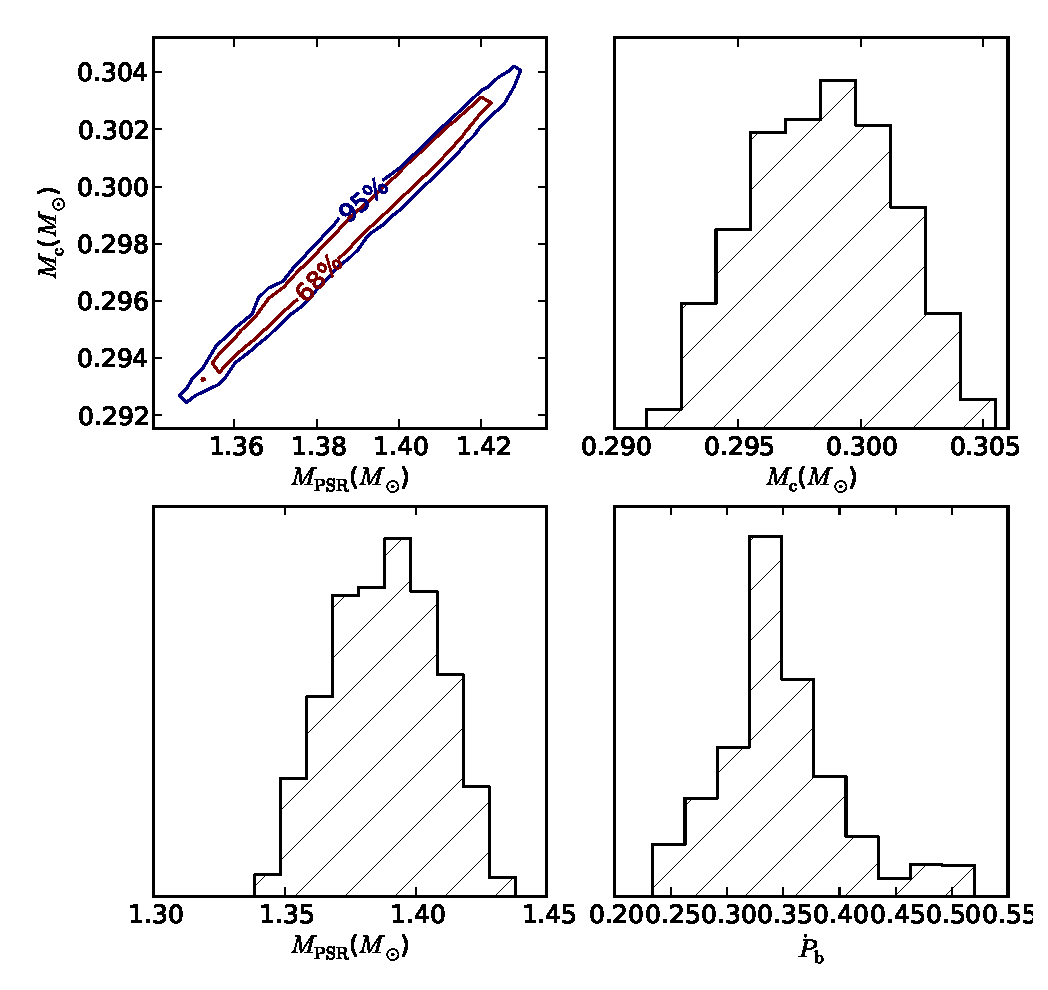
\includegraphics[width=4in]{masses.eps} \\ 
\caption {\label{fig:mass} Top left, top right and bottom left: the
  pulsar and companion masses as drawn from an MCMC simulation. Bottom right: MCMC distribution of $\dot{P}_{\rm b}$.} 
\end{figure} 

\begin{figure}
\includegraphics[width=4in]{DMX.ps} \\ 
\caption {\label{fig:dmx} The DM variation of PSR~J1713+0747. The DM plot is
separated into two segments with a small ``instrumental'' DM offset. This offset exists 
because the Mark~IV and ABPP TOAs (before MJD$\sim$53200) are extracted using
different pulse
profile templates from those used for ASP, GASP, GUPPI and PUPPI TOAs (after
MJD$\sim$53200). This template difference leads to a systematic
frequency-dependent arrival time shift. This shift is then absorbed by the DM
fitting and manifest a systematic DM offset. The dotted line shows the Solar
elongation of the pulsar. The subplot shows the structure
function (error bars) of the bottom half (i.e. last $\sim 9$~years) of DM
variation and its a power law fit (solid line). The best power law index is
0.74(8), different from the value of $5/3$ expected from a
``pure'' Kolmogorov medium. } 
\end{figure} 

%\begin{figure}
%\includegraphics[scale=0.6]{1713_TN.ps} \\ 
%\caption {\label{fig:TN} Black squares: The timing noise characteristic
%$\sigma_z(\tau)$ \citep{mte97} as a function of time scale $\tau$ calculated
%from the timing residuals of PSR~J1713+0747 obtained by setting $F_2=0$ and
%freezing all other parameters; shaded region:
%the distribution of $\sigma_z(\tau)$ calculated from 25 simulated timing residuals containing 
%Gaussian white noise of the same variance as the real residuals; hatched
%region: the distribution of $\sigma_z(\tau)$ calculated from simulated 
%residuals containing both Gaussian white noises and a
%random walk signal (red noise) which Gaussian random step sizes of
%$\sigma\simeq\sqrt{t_c/(1~{\rm yr})}\sigma_{\rm obs}$, where $t_c$ is the
%cadence of the simulated TOAs and $\sigma_{\rm obs}$ is the RMS of the
%observed timing residual.
%The simulated TOAs are uniformly distributed with a $t_c$ of 10 days.
%Here the step size of the random walk signal was chosen to simulate a red
%noise signal that grows to the same level of variance as the observed
%signal in $\sim$1 year.
%} 
%\end{figure} 


\begin{figure}
\includegraphics[scale=0.6]{1713_RN.ps} \\ 
\caption{\label{fig:TN}
Dots: residual RMS $\sigma^2_{\msR,2}$ from segments of the our data of length $T$.  
WN: theoretical residual expected from white noises of RMS 0.09$\mu$s; RW$_0$:
WN + random walk of phase; RW$_1$: WN + random walk of $\nu$; RW$_2$: WN +
random walk of $\dot{\nu}$. RW$_0$, RW$_1$, RW$_2$ are scaled such that they
produce an extra 0.1$\mu$s noise in 10 years.
} 
\end{figure} 

\begin{figure}
\includegraphics[width=4in]{FD.ps} \\ 
\caption {\label{fig:FD} GUPPI and PUPPI Post-fit residual versus frequency when fitted
without the FD model, showing the frequency dependency of the TOAs that is 
accounted for by the DM. For
clarity, this plot is made using only TOAs with error smaller than 3~$\mu$s.} 
\end{figure} 

\begin{figure}
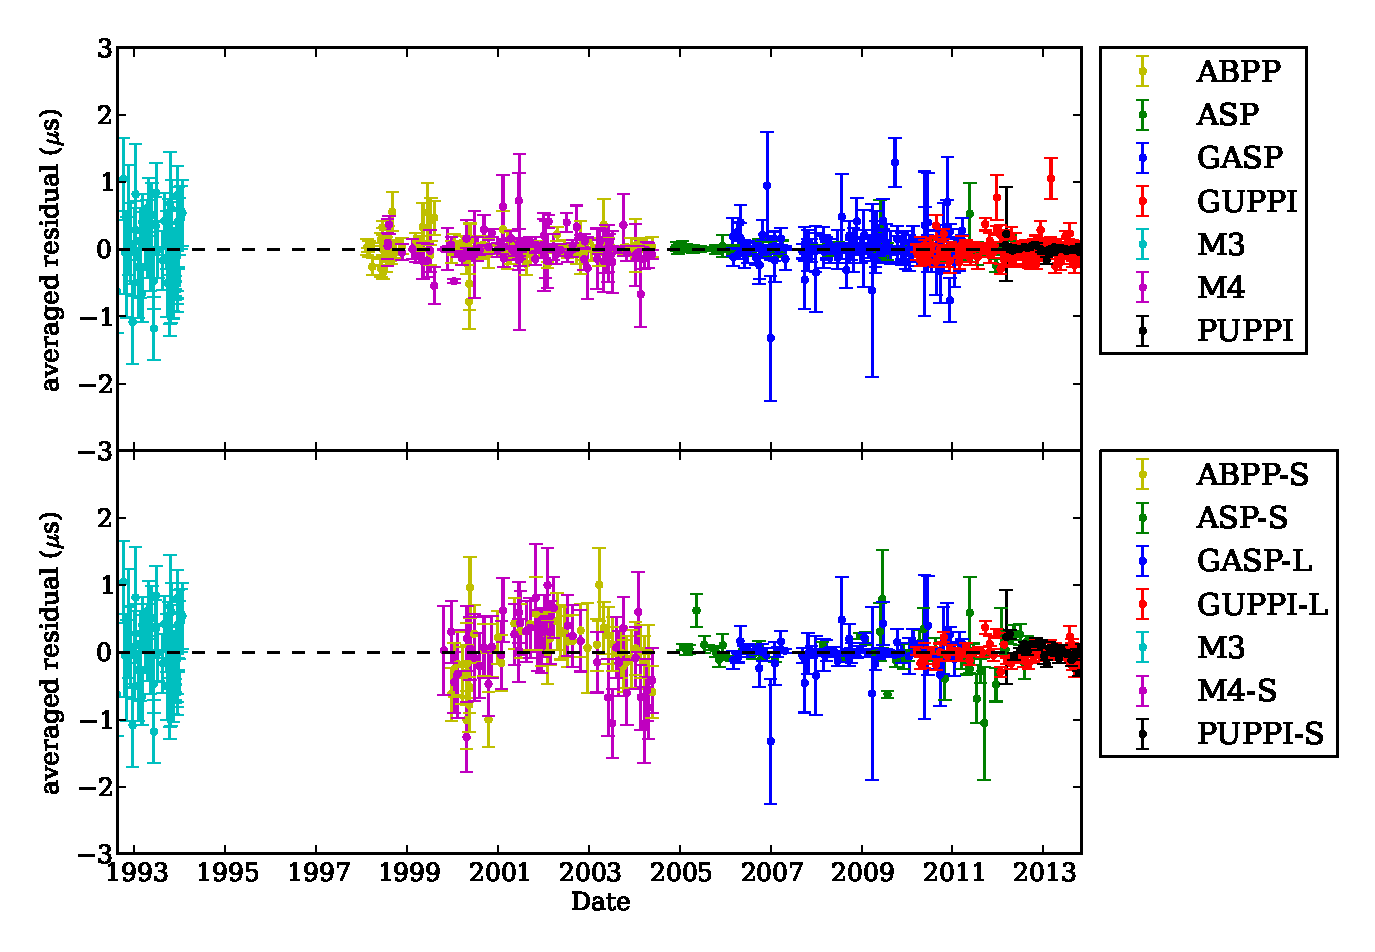
\includegraphics[width=4in]{residual.eps} \\ 
\caption {\label{fig:res} Top panel: The lower bands (1400-MHz for
Mark~IV, ABPP, ASP, and PUPPI, and 800~MHz for GASP and GUPPI) daily-averaged residuals of
J1713+0747. Bottom panel: The higher bands (2300~MHz for Mark4, ABPP, ASP, and PUPPI and
1400~MHz for GASP and GUPPI) residuals, showing the presence of some red noise.} 
\end{figure} 

\begin{figure}
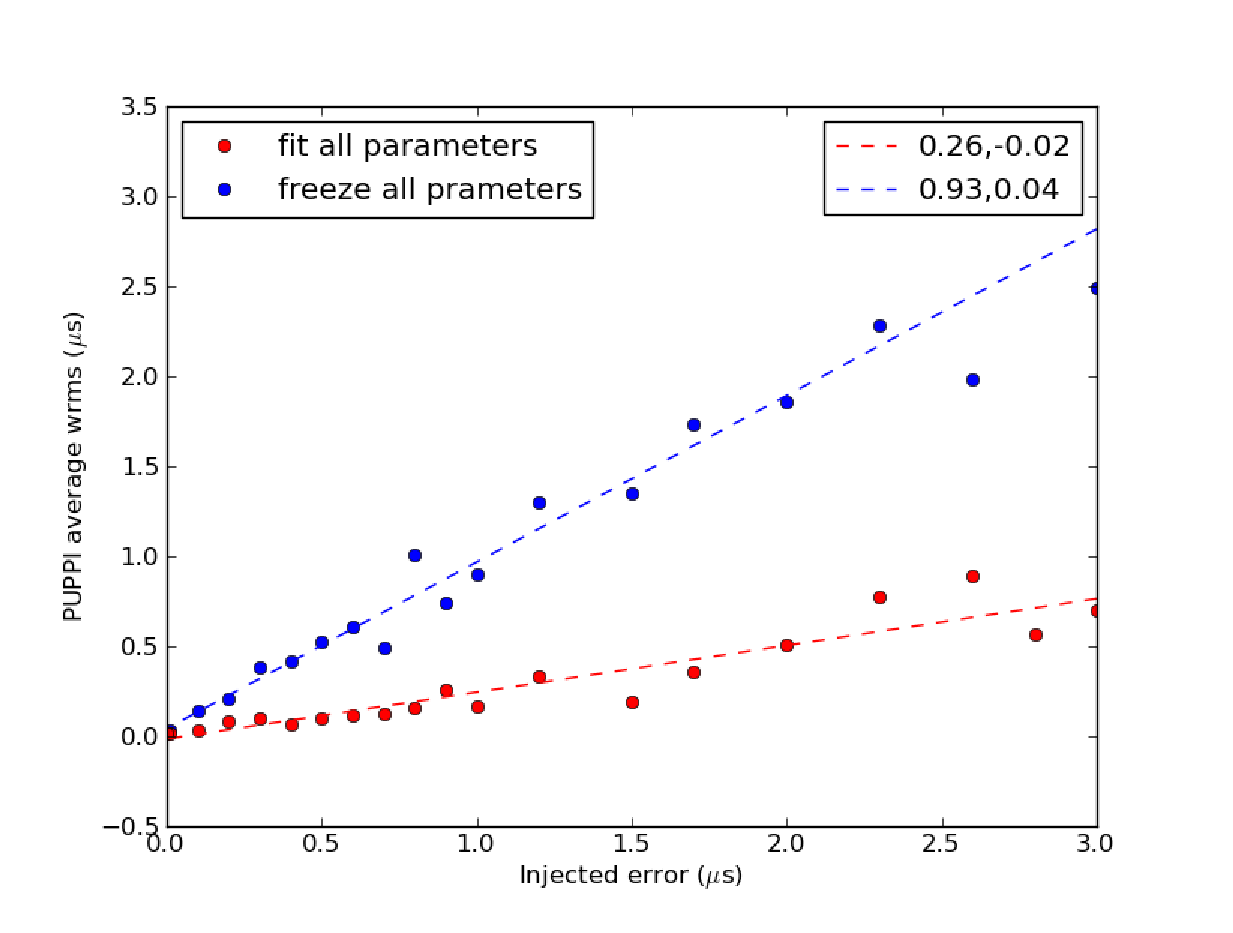
\includegraphics[width=4in]{overfit.eps} \\ 
\caption {\label{fig:overfit} Red points: post-fit residual WRMS as a function of the Gaussian
$\sigma$ of the  injected error; blue points: a control experiment:
post-fit residual WRMS as a function of injected error when freezing all fit
parameters. The dashed lines are the best linear fit to the points. Legends
show the best-fit slopes and intercepts. 
The blue points show a slope $\sim 1$,
indicating that almost 100\% of the injected errors are present in the
residuals, while only a fraction of that amount appears in the red residuals. 
This means that fitting the parameters absorbed part of the white noise.
} 
\end{figure} 

\begin{figure}
\includegraphics[width=8cm]{GdotContour.ps} \\ 
\caption {\label{fig:Gdot} Confidence contour of $\dot{G}$ and $\kappa_D$
calculated from PSRs~J1012+5307, J1738+0333, and J1713+0747 using an MCMC simulation.
The shaded area marks the 2$\sigma$ $\dot{G}$ limit from LLR. 
} 
\end{figure} 



%\clearpage
\begin{deluxetable}{lccccc}

\tabletypesize{\footnotesize}
\tablewidth{0pt}
\tablecaption{\label{tab:obs} 21 year J1713+0747 observations. }
\tablehead{ \colhead{System}  &\colhead{Dates}  &\colhead{Number of}
&\colhead{Epochs}  &\colhead{Bandwidth} 
&\colhead{Typical Integration}\\
& & \colhead{ToAs} & &\colhead{(MHz)} &\colhead{Time (min)}
}
\startdata
Mark III (L)&  1992 Aug$-$1994 Jan&  55&  55&  40&  47\\
Mark IV (L)&  1998 Jul$-$2004 May&  81&  81&  10&  58\\
Mark IV (S)&  1999 Oct$-$2004 May&  44&  44&  10&  29\\
Mark IV-O\tablenotemark{*} (L)&  2004 Jun$-$2005 Mar&  22&  16&  10&  60\\
Mark IV-O\tablenotemark{*} (S)&  2004 Jun$-$2005 Jan&  8&  7&  10&  30\\
ABPP (L)&  1998 Feb$-$2004 May&  98&  89&  56&  60\\
ABPP (S)&  1999 Dec$-$2004 May&  46&  46&  112&  30\\
ASP (L)&  2005 Jan$-$2012 Jan&  990&  48&  64&  20\\
ASP (S)&  2005 Jan$-$2012 Mar&  668&  41&  64&  20\\
GASP (820)&  2006 Mar$-$2011 Jan&  997&  41&  64&  20\\
GASP (L)&  2006 Mar$-$2010 Jun&  863&  42&  64&  20\\
GUPPI (820)&  2010 Mar$-$2013 Oct&  3533&  49&  800&  20\\
GUPPI (L)&  2010 Mar$-$2013 Nov&  4381&  64&  800&  20\\
PUPPI (L)&  2012 Mar$-$2013 Nov&  1972&  26&  800&  20\\
PUPPI (S)&  2012 Mar$-$2013 Nov&  992&  24&  800&  20
\enddata

\tablenotetext{*}{Here Mark IV-O stands for the recently-processed Mark IV
data that overlap with ASP data.}

\end{deluxetable}

%\clearpage 



\clearpage
\begin{deluxetable}{lc}

\tabletypesize{\footnotesize}
\tablewidth{0pt}
\tablecaption{\label{tab:par} Timing model parameters\tablenotemark{a}. }
\tablehead{ \colhead{Parameter}  &\colhead{Value}   }
\startdata
\textit{Measured Parameters}&  \\
Right Ascension, $\alpha$ (J2000)&  17:13:49.5320247(8)\\
Declination, $\delta$ (J2000)&  7:47:37.506126(20)\\
Spin Frequecy $\nu$~(s$^{-1}$)&  218.81184385472585(10)\\
Spin down rate $\nu'$ (s$^{-2}$)&  $-4.083894(7)\times10^{-16}$\\
Proper motion in $\alpha$, $\nu_{\alpha}=\dot{\alpha}\cos \delta$ (mas~yr$^{-1}$)&  4.918(2)\\
Proper motion in $\delta$, $\nu_{\delta}=\dot{\delta}$ (mas~yr$^{-1}$)&  -3.908(3)\\
Parallax, $\pi$ (mas)&  0.83(3)\\
Dispersion Measure\tablenotemark{b} (pc~cm$^{-3}$)&  15.97005(13)\\
$\sin i$, where $i$ is the orbital inclination angle&  0.949(4)\\
Orbital Period, $P_{\rm b}$ (day)&  67.8251298729(2)\\
Eccentricity, $e$&  0.0000749413(7)\\
Angle of periastron\tablenotemark{c}, $\omega$ (deg)&  176.1978(16)\\
Time of periastron passage, $T_0$ (MJD)&  53761.0330(3)\\
Change rate of $P_{\rm b}$, $\dot{P}_{\rm b}$ ($10^{-12}$s~s$^{-1}$)&  0.46(17)\\
Projected semi-major axis, $x$ (lt-s)&  32.34242185(14)\\
Change rate of projected semi-major axis $\dot{x}$ (lt-s~s$^{-1}$)&  0.00629(11)\\
Companion Mass, $M_c$ ($M_{\odot}$)&  0.290(14)\\
Profile frequency dependency parameter, FD1 &  -0.00016(3)\\
Profile frequency dependency parameter, FD2 &  0.00014(3)\\
Profile frequency dependency parameter, FD3 &  -0.000067(17)\\
Profile frequency dependency parameter, FD4 &  0.000015(5)\\
\textit{Fixed Parameters}&  \\
Solar system ephemeris&  DE421\\
Reference epoch for $\alpha$, $\delta$, and $\nu$ (MJD)&  53729\\
\textit{Derived Parameters}&  \\
Orbital inclination, $i$ (deg)&  71.6(7)\\
Position angle of ascending node, $\Omega$ (deg)&  90.1(9)\\
Pulsar mass, $M_{\rm PSR}$ ($M_{\odot}$)&  $1.3\pm0.1$\\
Dipole magnetic field, $B$ (G)&  $2.00\times10^{8}$\\
Characteristic age, $\tau_c$ (yr)&  $8.49\times10^{9}$
\enddata
\tablenotetext{a}{Numbers in parentheses indicate the uncertainties on the last digit(s).  Uncertainties on parameters are estimated from a general least square fit using {\sc tempo}.}
\tablenotetext{b}{The averaged DM value; See Section 3.2 and Figure 2 for the more discussion.}
\tablenotetext{c}{See Figure 2 of \citealt{sns+05} for definition.}


\end{deluxetable}

\clearpage 



\clearpage
\begin{deluxetable}{lcc}

\tabletypesize{\footnotesize}
\tablewidth{0pt}
\tablecaption{\label{tab:wrms}  }
\tablehead{ \colhead{Instrument-Backend}  &\colhead{WRMS (ns)}  &\colhead{`rescaled' WRMS (ns)}   }
\startdata
overall&  81&  $\sim245$\\
GASP-800&  141&  $\sim342$\\
GASP-L&  88&  $\sim131$\\
GUPPI-800&  202&  $\sim337$\\
GUPPI-L&  104&  $\sim165$\\
ASP-S&  88&  $\sim170$\\
ASP-L&  51&  $\sim104$\\
PUPPI-S&  46&  $\sim139$\\
PUPPI-L&  13&  $\sim102$
\enddata


\end{deluxetable}

\clearpage 


\end{document}


